\chapter{Enllaç Químic}

Una reacció química no és més que un procés que canvia l'ordenació d'enllaços del conjunt d'àtoms que conformen un sistema químic.
Això mostra la necessitat d'entendre aquest enllaç químic amb cert detall.
Hi ha tres conceptes clau en aquesta comprinesió del fenòmen de l'enllaç químic:
\begin{itemize}
\item D'entrada, ja el 1850 es va concebre el concepte de "valència" com la capacitat de combinació d'un element: el número d'àtoms d'Hidrogen o de Clor amb qui ho fa. 
En avançar cap a l'explicació dels sistemes químics en termes electrònics, usem el terme "electró de valència" com al número d'electrons que estan feblement units al nucli de l'àtom i que, per tant, poden formar part d'enllaços químics.
\item Els enllaços es formen perquè permeten els àtoms assolir estats de menor energia.
\item Les molècules adopten una certa geometria
\end{itemize}

Aquest capítol, basat en \cite{Mahan1977}, tracta de formular una teoria que expliqui aquests fenòmens.

\section{Parametritzant l'estructura molecular}

\subsection{Energies d'enllaç}

Es defineix com el canvi d'entalpia (calor específica a pressió constant) durant la separació d'una molècula gasosa en àtoms gasosos:\footnote{Per convertir entre unitats, pots usar \linkurl{http://www.colby.edu/chemistry/PChem/Hartree.html}}
\[
\ch{H2_{(g)} -> 2 H_{(g)}}, \; D(\ch{H-H})=\Delta H = 104 kcal/mol
\]
Aquesta $D$ també es pot avaluar en molècules poliatòmiques, i en aquest cas l'entorn molecular fa que hi pugui haver diferències entre les energies d'enllaç de dos elements determinats. No obstant això, aquestes diferenències són relativament menors:
\begin{eqnarray}
\ch{CH4_{(g)} -> CH3_{(g)} + H_{(g)}}, & D(\ch{H-CH3})=103 kcal/mol\\
\ch{CH3CH3_{(g)} -> CH3CH2_{(g)} + H_{(g)}}, & D(\ch{H-CH2CH3})=96 kcal/mol\\
\ch{(CH3)3CH_{(g)} -> (CH3)3C_{(g)}+H_{(g)}}, & D(\ch{H-C(CH3)3})=90 kcal/mol
\end{eqnarray}
\begin{figure}[h]
\centering
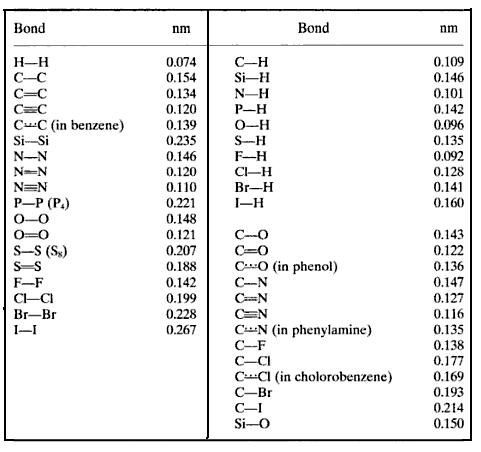
\includegraphics[scale=0.5]{figures/bond-energy-table.png}
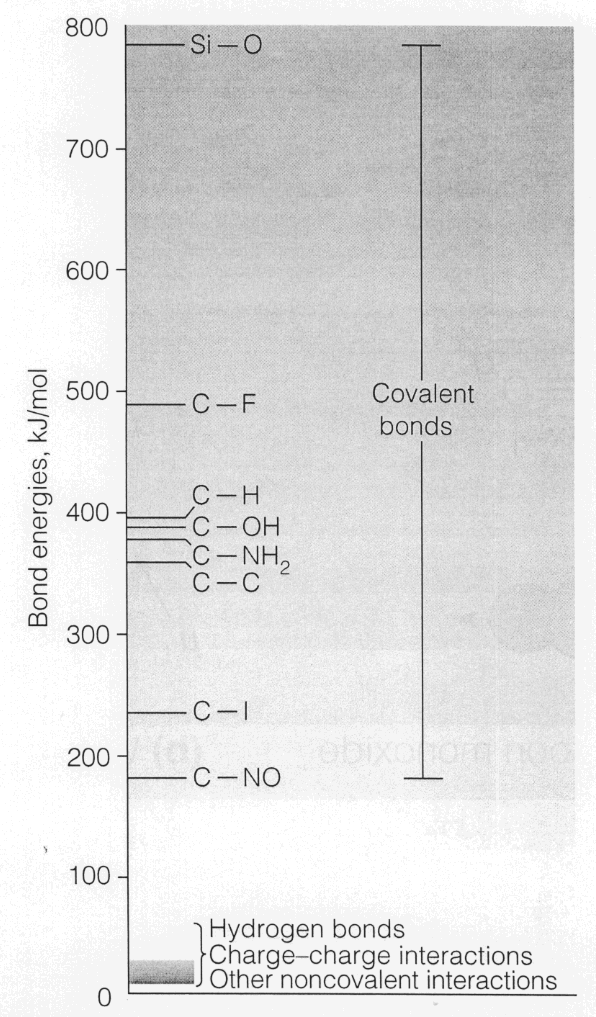
\includegraphics[scale=0.3]{figures/bonde.png}
\caption{Algunes energies d'enllaç típiques.}
\label{fig:bond-energy-table}
\end{figure}

\begin{figure}[h]
\centering
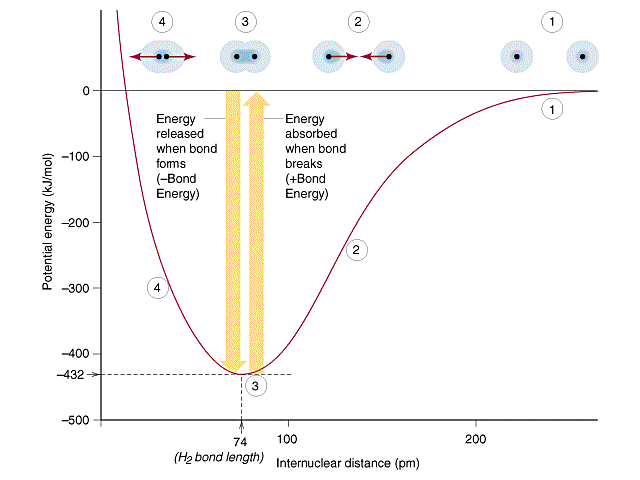
\includegraphics[scale=0.5]{figures/ebondh2.png}
\caption{Descripció del concepte energia d'enllaç}
\label{fig:bond-energy-table}
\end{figure}

\begin{exr}
Tenint en compte aquestes energies d'enllaç:

\begin{tabular}{cc}
& $E_b$ / kJ mol$^{-1}$ \\
\hline
C-O al monòxid de carboni & +1077 \\
C-O al diòxid de carboni & +805 \\
O-H & +464 \\
H-H & +436 \\
\hline
\end{tabular}

Calcula l'entalpia de la reacció:
\ch{CO_{(g)} + H2O_{(g)} -> CO2_{(g)} + H2_{(g)}} 
\end{exr}

Es poden determinar energies d'enllaç promig a partir d'aquestes observacions:
\begin{table}[h!]
  \begin{center}
    \caption{Energies d'enllaç promig en kcal mol$^{-1}$\cite{Mahan1977}}
    \label{tab:bonde}
    \begin{tabular}{cccc}
      \hline
      Enllaç & $\bar{D}$ & Enllaç & $\bar{D}$\\
      \hline
      \ch{C-H} & 98.7 & \ch{C-C} & 82.6 \\
      \ch{C-F} & \approx 110 & \ch{C=C} & 145.8 \\
      \ch{C-Cl} & 80 & \ch{C+C} & 199.6 \\
      \ch{C-Br} & 69 & \ch{C-O} & 85 \\
      \ch{C-I} & 55 & \ch{C=O} & 178 \\
      \ch{C-N} & 80 & \ch{O-H} & 110.6 \\
      \hline
    \end{tabular}
  \end{center}
\end{table}

\begin{exr}
Fent servir les dades de la Taula \ref{tab:bonde}, estima l'energia alliberada a pressió constant en la reacció:
\[
\ch{H2_{(g)}+Cl2_{(g)} + C_{(grafit)} -> CH3Cl_{(g)}}
\]
si la calor de vaporització del grafit a àtoms de carboni és de 170.9 kcal mol$^{-1}$.
\end{exr}

\subsection{Longituds i angles d'enllaç}

Els enllaços vibren constantment per la $T$ no nul·la de les molècules.
No obstant això, podem mesurar distàncies d'enllaç promig que es pot mesurar a partir d'estudis de raigs X o l'espectroscopia molecular (Taula \ref{tab:bonddist}).
\begin{table}[h!]
  \begin{center}
    \caption{Energies d'enllaç promig en kcal mol$^{-1}$\cite{Mahan1977}}
    \label{tab:bonddist}
    \begin{tabular}{cccc}
      \hline
      Enllaç & BD / \AA & Enllaç & BD / \AA \\
      \hline
      \ch{F2}  & 1.42 & \ch{HF} & 0.92 \\
      \ch{Cl2} & 1.99 & \ch{HCl} & 1.27 \\
      \ch{Br2} & 2.28 & \ch{HBr} & 1.41 \\
      \ch{I2}  & 2.67 & \ch{HI} & 1.61 \\
      \ch{ClF} & 1.63 & \ch{H2} & 0.74 \\
      \ch{BrCl} & 2.14 & \ch{N2} & 1.094 \\
      \ch{BrF} & 1.76 & \ch{O2} & 1.207 \\
      \ch{ICl} & 2.32 & \ch{NO} & 1.151 \\
       &  & \ch{CO} & 1.128 \\
      \hline
    \end{tabular}
  \end{center}
\end{table}
Els valors de la taula són molt constants a totes les molècules que contenen aquests enllaços, fins i tot més que no pas el que succeïa amb les energies d'enllaç promig de la Taula \ref{tab:bonde}. Quan això no es compleix és perquè hi ha enllaços diferents (dobles, triples...). Per exemple, entre l'età (\ch{C2H6}), l'etilè (\ch{C2H4}) i l'acetilè (\ch{C2H2}) les energies d'enllaç entre els àtoms de C varien de 83 a 146 i 200 kcal mol$^{-1}$, i les distàncies de 1.54 a 1.34 i 1.20, respectivament.


També es dóna constància en les geometries de les molècules, com s'aprecia a la Figura \ref{fig:molecular-geometry}.

\begin{figure}[h]
\centering
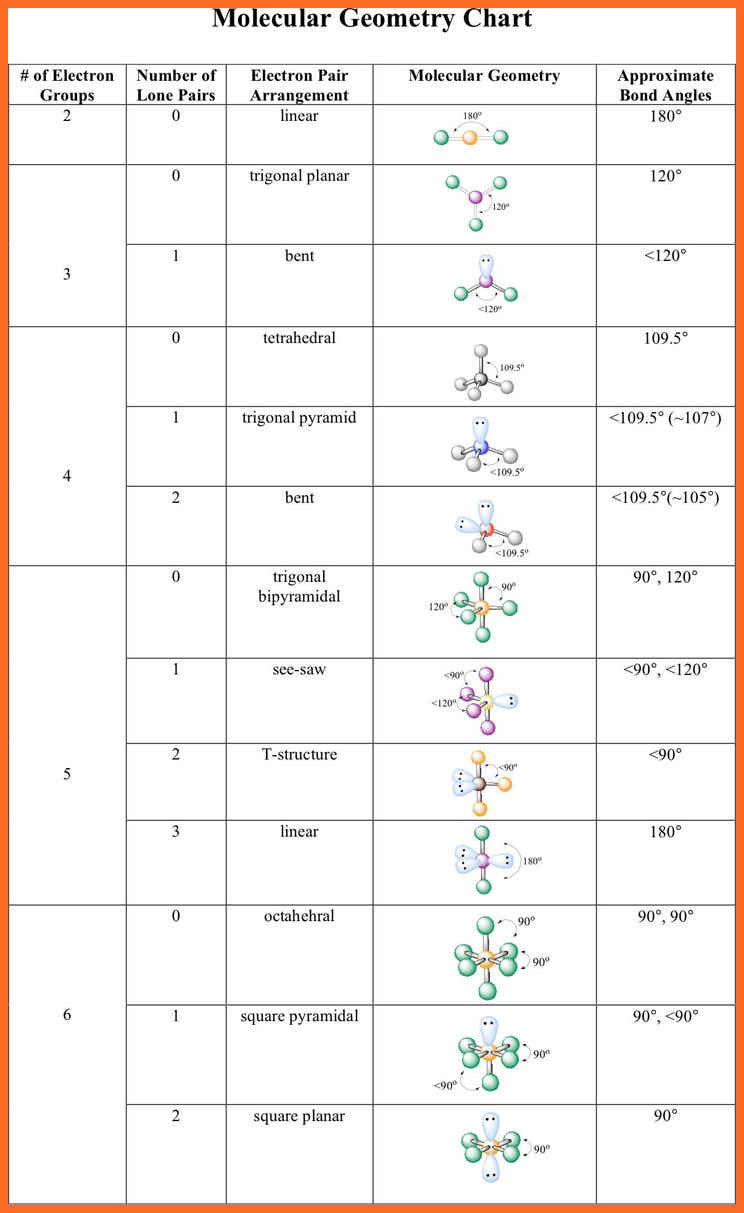
\includegraphics[scale=0.5]{figures/molecular-geometry.png}
\caption{Estructures moleculars típiques, mostrant alguns angles d'enllaç rellevants}
\label{fig:molecular-geometry}
\end{figure}

\subsection{Espectroscopia molecular}

De la mateixa manera que en una molècula els nivells electrònics estan quantitzats (amb intèrvals energètics de l'ordre de 100 kcal mol$^{-1}$), ho estàn també els nivells vibracionals (on $E_{vib}=(v+\frac{1}{2})h\nu$, on $v$ és el nñúmero quàntic vibracional; amb intèrvals de 1-7 kcal mol$^{-1}$) i rotacionals ($\Delta E_{rot}=h \nu = \frac{\hbar}{2I}[J(J+1)-J'(J'+1)]$, on $J$ és el número quàntic rotacional i $I$ és el moment d'inèrcia de la molècula; amb intèrvals de menys de 0.03 kcal mol$^{-1}$) (veure la Figura \ref{fig:ERVlevels}).
\begin{figure}[h]
\centering
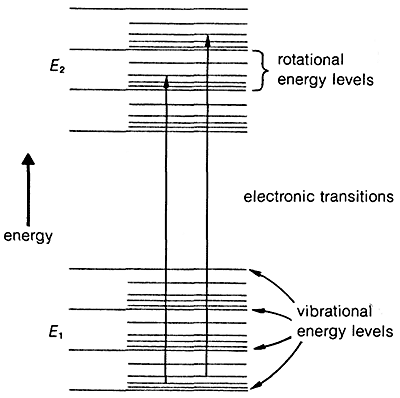
\includegraphics[scale=0.3]{figures/EVRlevels.png}
\caption{Estructures moleculars típiques, mostrant alguns angles d'enllaç rellevants}
\label{fig:EVRlevels}
\end{figure}

L'espectroscopia molecular analitza la interacció de la llum amb les molècules i n'extreu característiques geomètriques a partir d'analitzar les frequències d'absorció/emissió.
Cada característica es pot estudiar amb una banda determinada de l'espectre lumínic (F.
\begin{figure}[h]
\centering
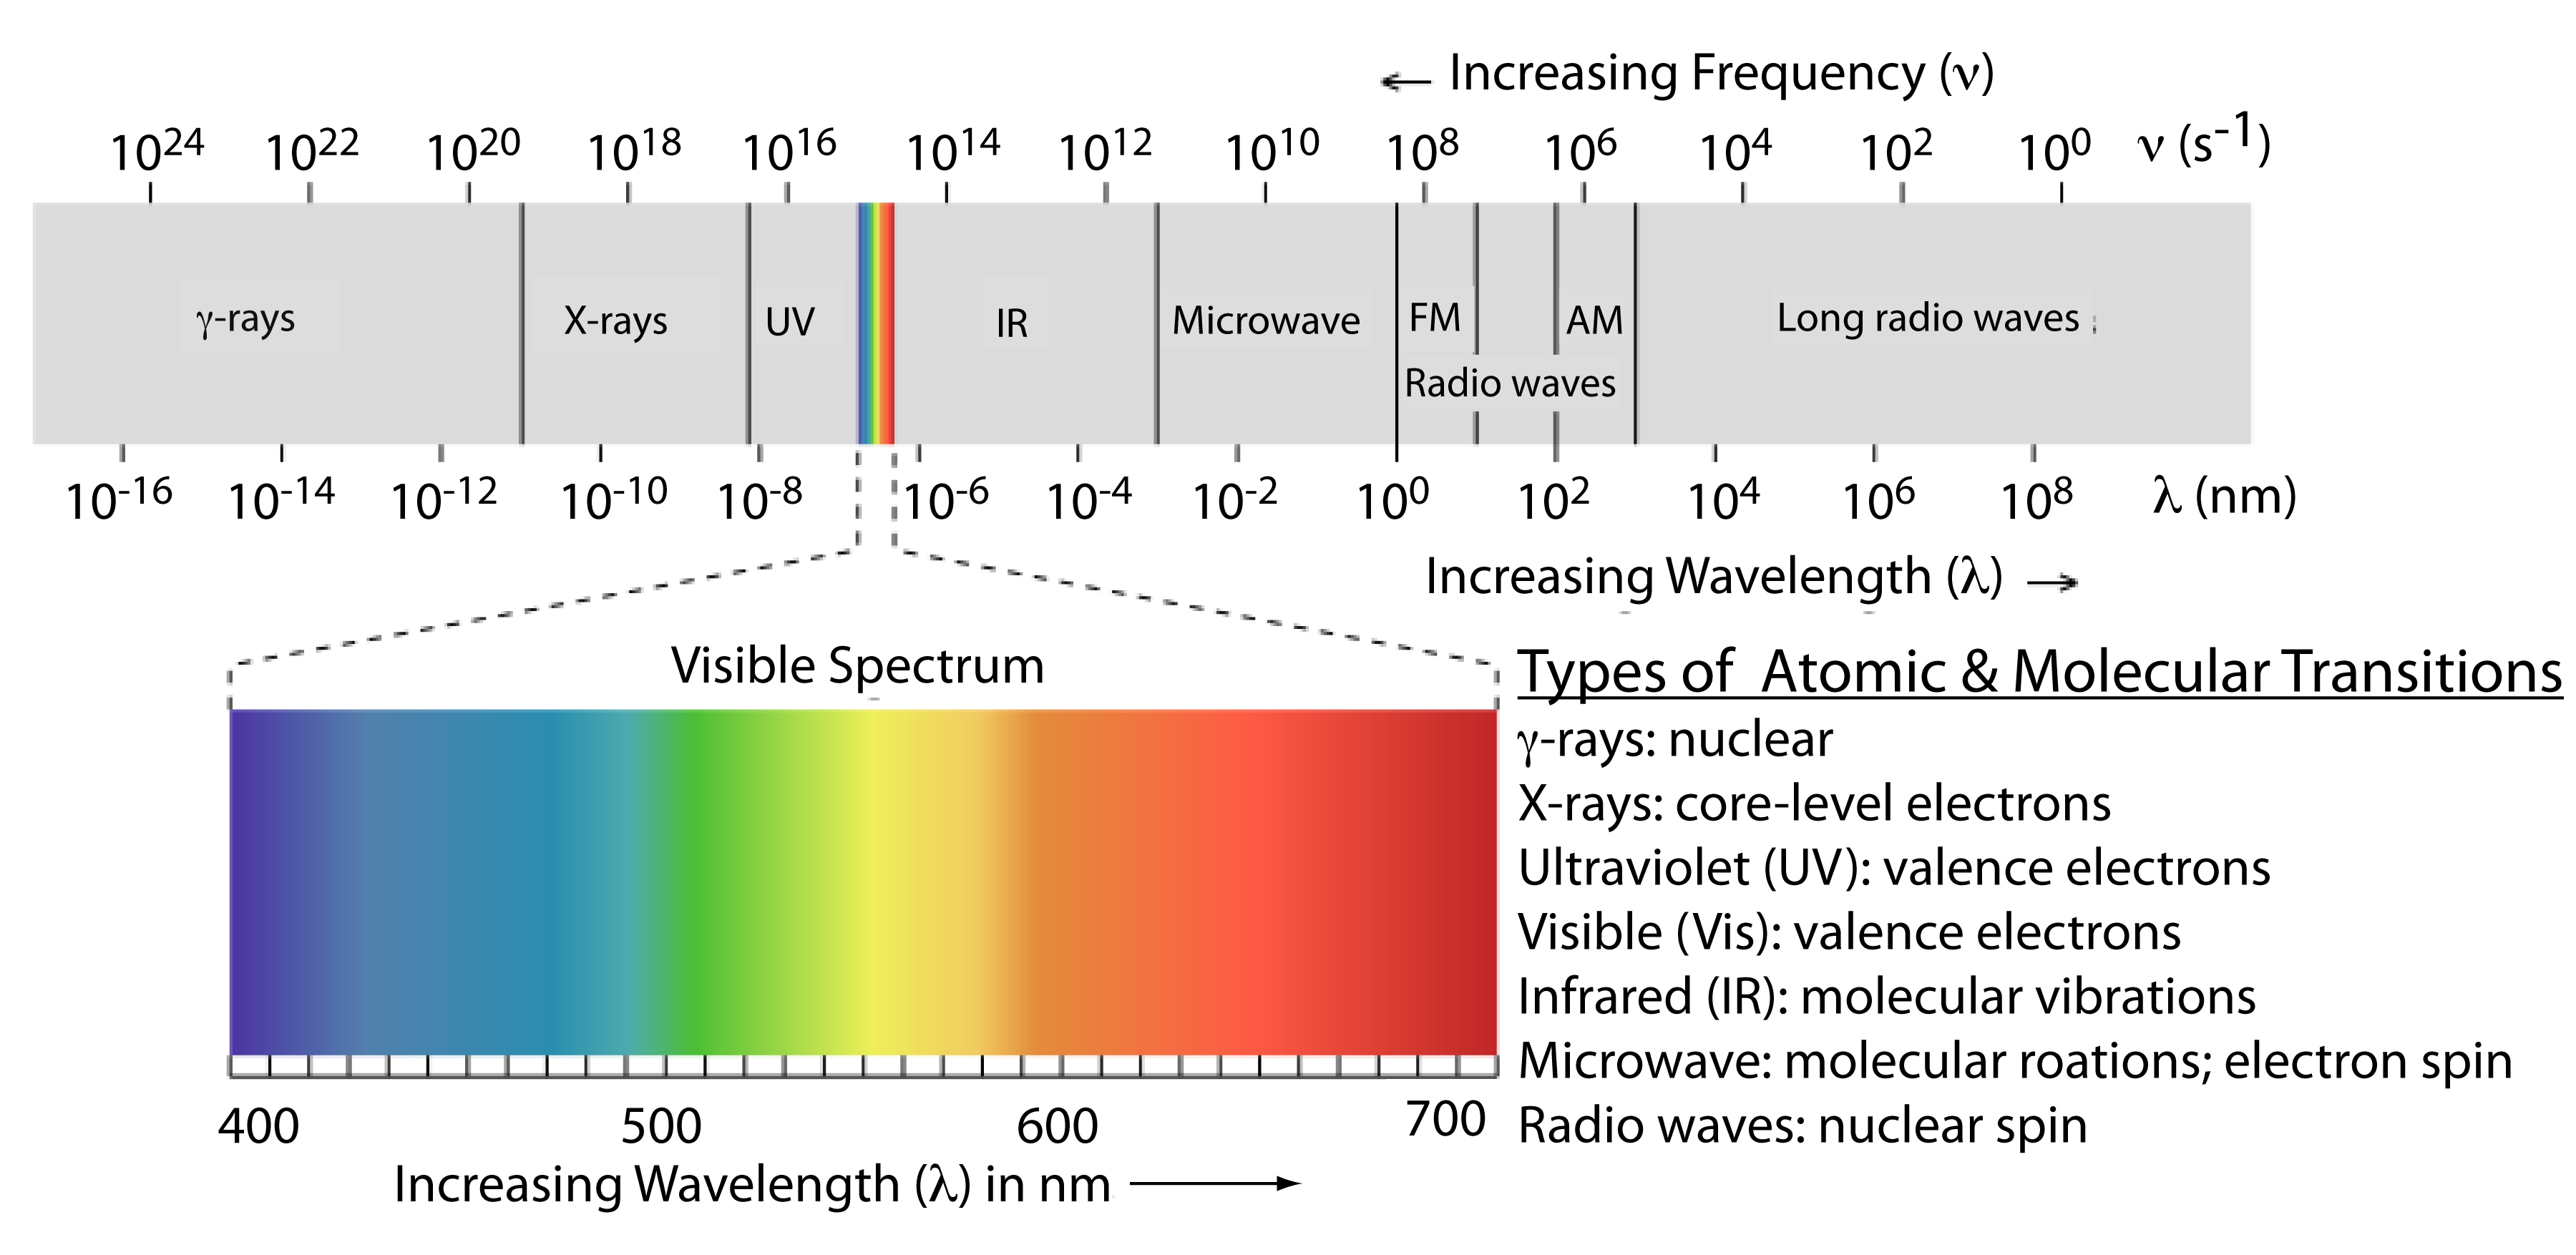
\includegraphics[scale=0.5]{figures/MolSpect.png}
\caption{Espectre electromagnètic i nivells d'energia molecular que es veuen afectats.}
\label{fig:MolSpect}
\end{figure}

\section{Tipus d'enllaç}
És útil usar uns models conceptuals que expliquin l'estructura molecular. Són models extrems que no sempre es segueixen de manera exacta per les substàncies químiques. Sovint tenim barreges d'aquests models en un sistema real, però serveixen per conceptualitzar la manera en què la matèria s'organitza a nivell molecular i atòmic.

La majoria dels enllaços químics tenen propietats intermèdies entre el covalent i l'iònic però estan força aprop d'algun dels dos models.

\subsection{Enllaç covalent}

%aquesta secció està incompleta i necessita un desenvolupament a partir de l'experiència a classe

\begin{mdframed}[backgroundcolor=gray!30,frametitle=Estructura molecular i enllaç covalent]
En aquesta secció explorem el concepte d'orbital molecular i d'estructura molecular covalent. Usarem alhora els conceptes d'orbitals $\sigma$ i $\pi$ (provinents de la teoria d'orbitals moleculars) amb el model de Pauling de promoció i hibridació.
\end{mdframed}

\begin{exr}
Sabries explicar perquè la rotació en la molècula d'etilè (\ch{C2H4}) és més costosa energèticament que la rotació en la molècula d'età (\ch{C2H6})?
\end{exr}

%\subsection{Enllaç metàlic}
\subsection{Enllaç iònic}

Tot i que, com hem vist, l'estructura electrònica d'un àtom és complexa, podem pensar que des de la distància la distribució dels electrons segueix una forma propera a esfèrica. Per tant, i seguint la llei de Coulomb, aquestes esferes es comporten com si la seva càrrega estigués concentrada al seu centre, i podem considerar els ions com a càrregues puntuals.

En el cas del clorur de sodi (\ch{NaCl}), l'espectroscopia de raigs X mostra que l'estructura del compost és regular amb esferes que contenen 10 i 18 e$^{-}$ cadascuna, corresponents als ions \ch{Na+} i \ch{Cl-}, respectivament. Això demostra que els ions existeixen i que, per tant, les forces que uneixen aquests ions han de ser, per força, elèctriques.

Podem avaluar l'energia de la formació del compost iònic \ch{NaCl} a partir del cicle termodinàmic  (cicle Born-Haber):

%\schemestart
%  \ch{C\sld{} + 2 H2O\gas}
%  \arrow{->[\SI{90.1}{\kilo\joule}]}[,1.5]
%  \ch{CO2\gas{} + 2 H2\gas}
%  \arrow{<-[][*{0.north west}\SI{-393.5}{\kilo\joule}]}[-125,2]
%  \ch{C\sld{} + 2 H2\gas{} + O2\gas}
%  \arrow(@c3--@c1){->[][*{0.north east}\SI{-483.6}{\kilo\joule} ]}
%\schemestop

\begin{center}
\schemestart
  \ch{Na\gas{} + Cl\gas}
  \arrow{->[I(\ch{Na})-A(\ch{Cl})]}[,1.5]
  \ch{Na+ \gas{} + Cl- \gas}
  \arrow{->[][*{0.east}$U$]}[-90,2]
  \ch{NaCl\sld}
  \arrow{<-[][*{0.north}$\Delta H_f(\ch{NaCl})$]}[180,2]
  \ch{Na\sld{} + 1/2 Cl2\gas}
  \arrow{->[][*{0.east}$\begin{array}{c}\Delta H_{vap}(\ch{Na})\\+\frac{1}{2}D(\ch{Cl2})\end{array}$]}[90,2]
\schemestop
\end{center}
 
%\begin{mdframed}[backgroundcolor=gray!30,frametitle=Llei de les proporcions definides]
%En un compost donat, els elements constituients es combinen sempre en les mateixes proporcions pondarebles, sigui quin sigui l'origen i el mode de preparació dels compostos.
%\end{mdframed}

\begin{exr}
Se sap que una molècula gasosa de \ch{NaCl} té una distància interatòmica de 2.38\AA. Quina és l'energia potencial Coulòmbica d'un mol d'aquestes molècules?
\end{exr}

A partir del resultat de l'anterior exercici, i tenint en compte altres dades experimentals, podem veure que la formació d'un mol de molècules de \ch{NaCl} implica les següents relacions energètiques: 
\[
\begin{array}{cc}
\begin{array}{c}
\ch{Na \gas-> Na+ \gas{} + e-}\\
\ch{e- + Cl \gas{} -> Cl- \gas{}}\\
\hline
\ch{Na + Cl -> Na+ \gas{} + Cl- \gas}\\
\\
\ch{Na+ \gas{} + Cl- \gas -> NaCl\gas}\\
\hline
\ch{Na \gas{} + Cl \gas -> NaCl\gas}
\end{array}
\quad
\begin{array}{c}
\Delta E=I(\ch{Na}) = 118.4 \km \\
\Delta E=-A(\ch{Cl}) = -83.4 \km\\
\hline
\Delta E= 35\km \\
\\
\Delta E = -139.3 \km\\
\hline
\Delta E = -104.3 \km
\end{array}
\end{array}
\]
L'esquema ens mostra que, d'entrada, els ions no tendiran per ells mateixos a formar-se, i necessiten de l'energia que es desprèn en formar les interaccions Coulòmbiques entre aquests ions per tal de que sigui favorable.

No obstant, ens interessa entendre com es formen els cristalls de \ch{NaCl}. De fet, aquests cristalls tenen pressions de vapor extremadament baixes i, per tant, difícilment trobarem aquestes molècules gasoses. Per a calcular quanta energia es desprèn en formar aquests sòlids  hem de tenir en compte l'entalpia de malla $\Delta H_L$. Aquesta és, per al cas que ens ocupa,  a l'entalpia molar estàndar (1 atm i 0$\degree$C) del procés  \ch{NaCl\sld -> Na+ \gas{} + Cl- \gas}.
A $T=0K$, $\Delta H_L=U_L$, l'energia de malla, que només depèn de les interaccions Coulòmbiques dels ions. A $T$ normals, la diferència entre les dues és relativament menor.

Fem un càlcul d'aquesta energia potencial. Imaginem una disposició lineal d'ions positius i negatius amb càrregues $+z$ i $-z$, respectivament, separats per una distància $d$. L'energia potencial del primer ió seria:
\begin{eqnarray}
E_p&=&\frac{1}{4\pi \varepsilon_0} \times \left(
-\frac{z^2e^2}{d}+\frac{z^2e^2}{2d}-\frac{z^2e^2}{3d}+\frac{z^2e^2}{4d}-\cdots
\right)\\
&=&\frac{z^2e^2}{4\pi \varepsilon_0 d}\times \underbrace{(-1+\frac{1}{2}-\frac{1}{3}+\frac{1}{4}-\cdots)}_{-\ln 2}\\
&=&-\frac{z^2e^2} \ln 2
\end{eqnarray}
Quantitat que haurem de multiplicar per 2 per tal de considerar els dos costats de l'ió, així com per $N_A$ per tal d'obtenir el valor molar.
Finalment, podríem generalitzar el resultat per a qualsevol xarxa d'ions de càrregues de diferent signe $z_A$ i $z_B$, tot obtenint el resultat:
\[
E_p=-A\frac{|z_A z_B|N_A e^2}{4\pi \varepsilon_0 d}
\]
on $A$ és la constant de Madelung, que depèn de l'estructura tridimensional del cristall (per al \ch{NaCl}, $A=1,748$).

No obstant, aquesta no és l'única contribució a l'energia de malla, ja que cal incorporar el solapament que es produeix entre els orbitals dels dos ions quan s'apropen. Aquesta és proporcional al factor $\exp{-\frac{d}{d^*}}$, on $d^*$ es pren amb valor 34.5pm.

Si sumem les dues contribucions i trobant-ne el mínim, obtenim l'equació de Born-Mayer:
\begin{equation}
E_{p,min}=-\frac{N_A|z_A z_B| e^2 }{4\pi \varepsilon_0 d}\left(1-\frac{d^*}{d}\right) A
\label{eq:BornMayer}
\end{equation}

\begin{exr}
Dedueix l'equació de Born-Mayer a partir de considerar, de forma simplificada, que l'energia d'atracció Coulòmbica es pot expressar com $-\frac{Me^2}{r}$ i que la repulsió entre ions es pot expressar com $\frac{B}{r^n}$.
%U=-\frac{Me^2}{r_0}(1-1/n)
\end{exr}
\begin{exr}
L'òxid de magnesi, \ch{MgO}, té la mateixa estructura que el \ch{NaCl}. Sabent que $r(\ch{Mg^{2+}})=72pm$ i que $r(\ch{O^{2-}})=140pm$, calcula l'energia de malla d'aquest compost iònic.
%\includegraphics[scale=0.5]{figures/res_ex1.png}
%-3.84 10^3 kj mol-1
\end{exr}

\begin{exr}
Fent servir el cicle de Born-Haber, estima l'entalpia de malla del \ch{KCl}.
%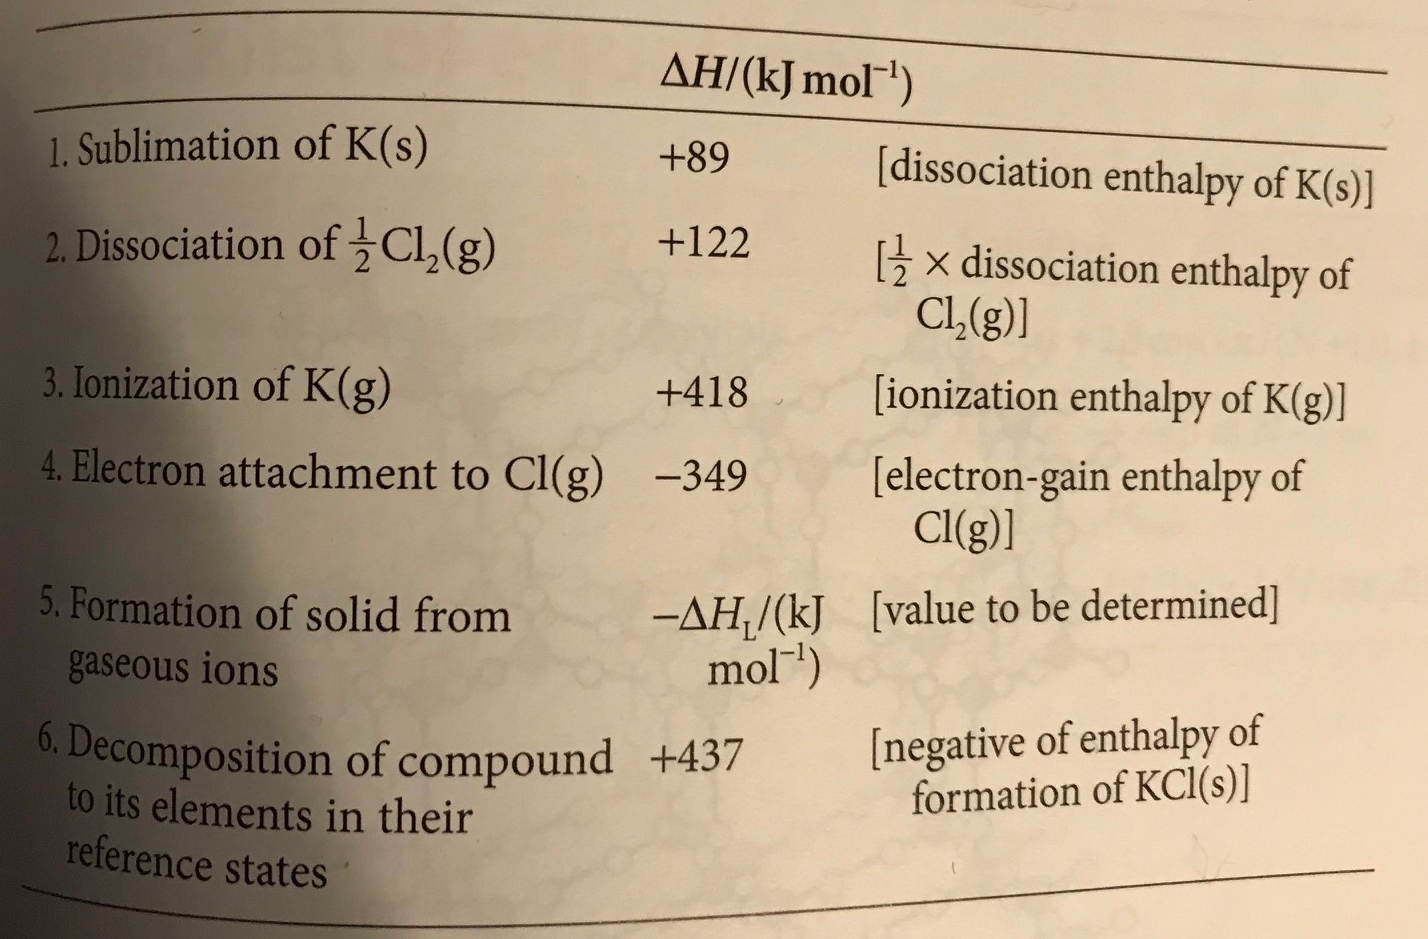
\includegraphics[scale=0.5]{figures/res_ex2.png}
%717 kj mol-1
%exercici examen CaO (veure atkins)
\end{exr}

%
%\section{Orbitals atòmics i moleculars}
%
%\section{La química d'elements rellevants}
%\subsection{Hidrògen}
%\subsection{Nitrògen}
%\subsection{Oxigen, sofre}
%\subsection{Carboni}
